%! Suppress = MissingImport
%TODO: dodać screeny testów i krótkie opisy
\subsection{Testy modułu}\label{subsec:module-tests}
\begin{figure}[h]
    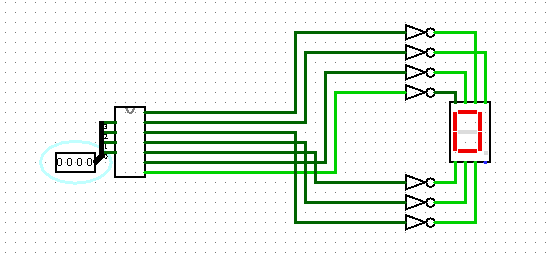
\includegraphics[width=\linewidth]{ScreenshotsTests/Comp 1/Comp 1_00009.png}
    \caption{Test 1 - (binary) 0000, (decimal) 0}
    \label{fig:test0}
\end{figure}

Test 1 zakończony pomyślnie.

\begin{figure}[H]
    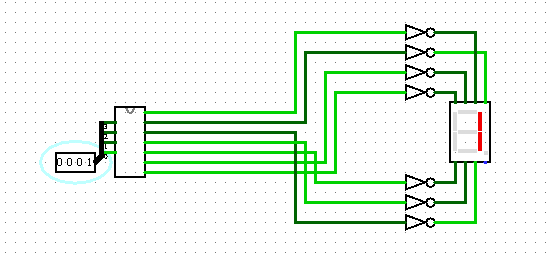
\includegraphics[width=\linewidth]{ScreenshotsTests/Comp 1/Comp 1_00008.png}
    \caption{Test 2 - (binary) 0001, (decimal) 1}
    \label{fig:test1}
\end{figure}

Test 2 zakończony pomyślnie.

\begin{figure}[H]
    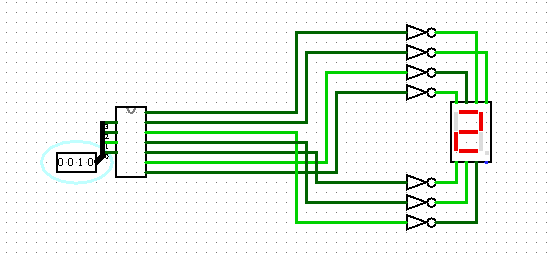
\includegraphics[width=\linewidth]{ScreenshotsTests/Comp 1/Comp 1_00007.png}
    \caption{Test 3 - (binary) 0010, (decimal) 2}
    \label{fig:test2}
\end{figure}

Test 3 zakończony pomyślnie.

\begin{figure}[H]
    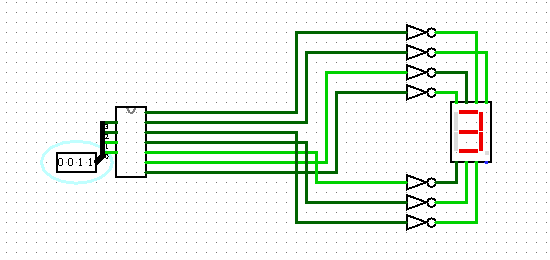
\includegraphics[width=\linewidth]{ScreenshotsTests/Comp 1/Comp 1_00006.png}
    \caption{Test 4 - (binary) 0011, (decimal) 3}
    \label{fig:test3}
\end{figure}

Test 4 zakończony pomyślnie.

\begin{figure}[H]
    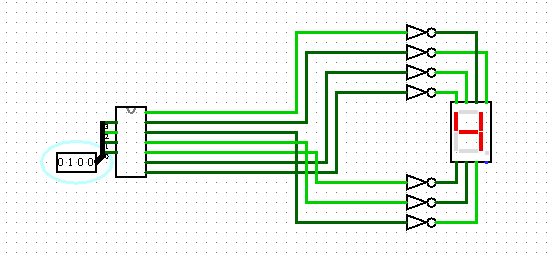
\includegraphics[width=\linewidth]{ScreenshotsTests/Comp 1/Comp 1_00005.png}
    \caption{Test 5 - (binary) 0100, (decimal) 4}
    \label{fig:test4}
\end{figure}

Test 5 zakończony pomyślnie.

\begin{figure}[H]
    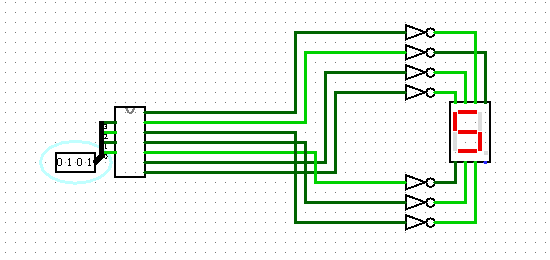
\includegraphics[width=\linewidth]{ScreenshotsTests/Comp 1/Comp 1_00004.png}
    \caption{Test 6 - (binary) 0101, (decimal) 5}
    \label{fig:test5}
\end{figure}

Test 6 zakończony pomyślnie.

\begin{figure}[H]
    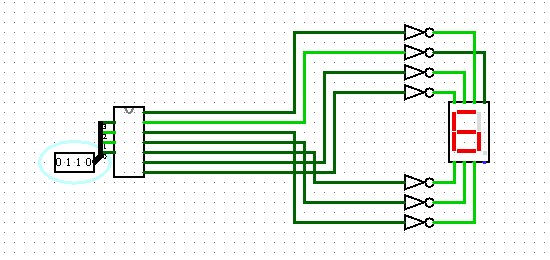
\includegraphics[width=\linewidth]{ScreenshotsTests/Comp 1/Comp 1_00003.png}
    \caption{Test 7 - (binary) 0110, (decimal) 6}
    \label{fig:test6}
\end{figure}

Test 7 zakończony pomyślnie.

\begin{figure}[H]
    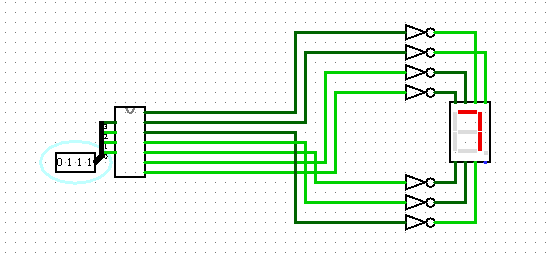
\includegraphics[width=\linewidth]{ScreenshotsTests/Comp 1/Comp 1_00002.png}
    \caption{Test 8 - (binary) 0111, (decimal) 7}
    \label{fig:test7}
\end{figure}

Test 8 zakończony pomyślnie.

\begin{figure}[H]
    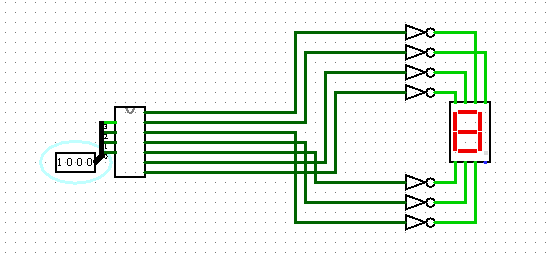
\includegraphics[width=\linewidth]{ScreenshotsTests/Comp 1/Comp 1_00001.png}
    \caption{Test 9 - (binary) 1000, (decimal) 8}
    \label{fig:test8}
\end{figure}

Test 9 zakończony pomyślnie.

\begin{figure}[H]
    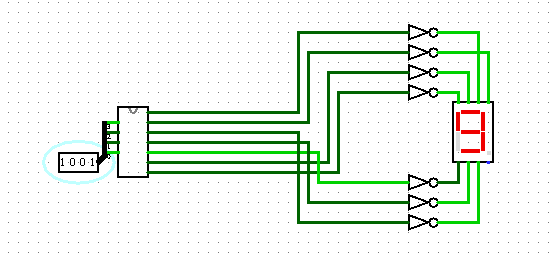
\includegraphics[width=\linewidth]{ScreenshotsTests/Comp 1/Comp 1_00000.png}
    \caption{Test 10 - (binary) 1001, (decimal) 9}
    \label{fig:test9}
\end{figure}

Test 10 zakończony pomyślnie.

\subsection{Ocena}\label{subsec:qa-review}
Moduł 7digit.circ spełnia założenia QA.